Antes de comenzar con el rendimiento de la red, es necesario saber cómo esta está dispuesta  y cuáles son las direcciones IP tanto de las interfaces interiores de la red 4G como de las interfaces correspondientes al usuario y al router. Esto se puede observar en la figura \ref{fig:EsquemaRed}.

\begin{figure}[H]
    \centering
    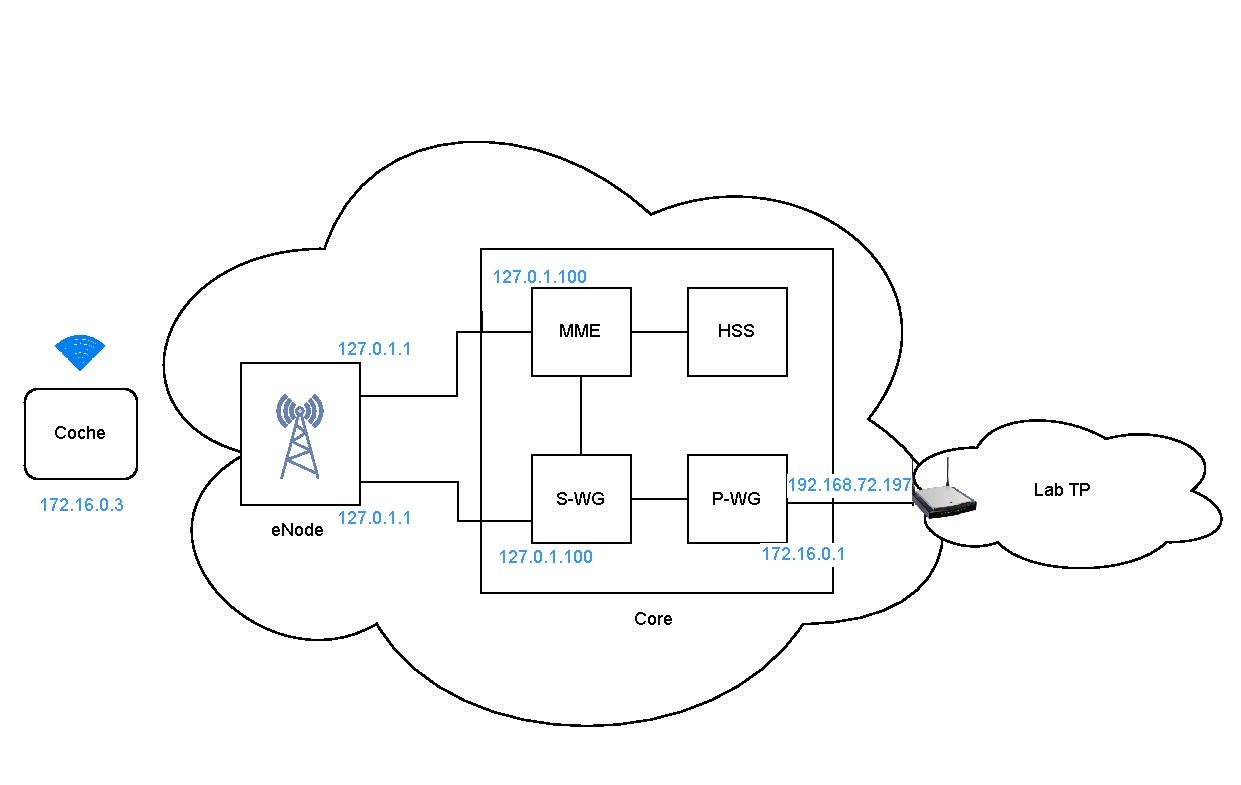
\includegraphics[width=0.99\textwidth]{Imagenes/Solucion/10.pdf}
    \caption{Esquema de la red. (Se ha usado \textit{iproute} para saber las direcciones IP de las diferentes interfaces).}
    \label{fig:EsquemaRed}
\end{figure}

Una de las formas más simples de calcular el rendimiento de la red \textbf{extremo a extremo} es usando la herramienta \textit{ping}. Esta herramienta mide la latencia enviando un paquete de datos desde un dispositivo a otro y midiendo el tiempo que tarda en ser recibido y respondido. La latencia se refiere al tiempo que tarda un paquete de datos en viajar desde un dispositivo a otro en una red.\\
Haciendo \textit{ping} desde nuestro equipo de usuario \footnote{Se ha hecho uso de la app “Ping IP”} (UE), con dirección IP 176.16.0.3, que corresponde a un dispositivo móvil  que se encuentra en la misma sala y red que el ordenador de sobremesa en el que corre el eNodeB y el core obtenemos \ref{fig:ping} 

 \begin{figure}[H]
    \centering
    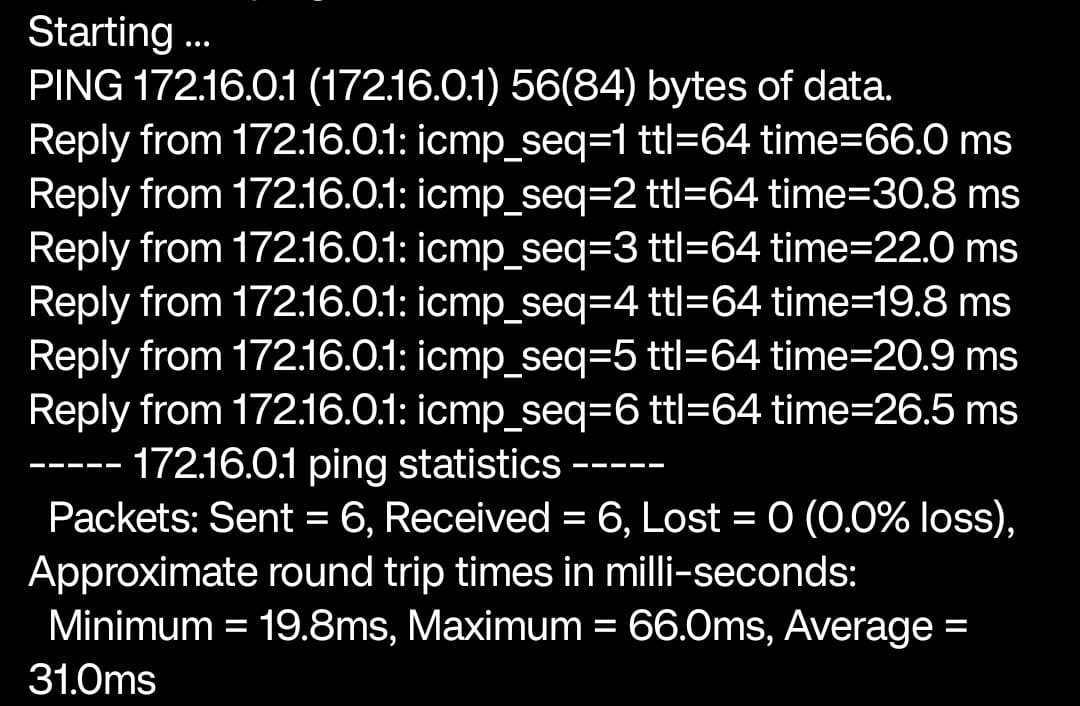
\includegraphics[width=0.53\textwidth]{Imagenes/Rendimiento/ping.jpeg}
    \caption{Salida del comando \textit{ping}.}
    \label{fig:ping}
\end{figure}

Aunque la latencia se puede ver afectada por la calidad de la red, la carga de tráfico, la distancia a la estación base, y otros factores, los valores obtenidos que se aprecian son bastante buenos. Se puede considerar que un buen valor de latencia en una red 4G se encuentra en el rango de 30 a 50 ms.\\
En lo que respecta al streaming de video (lo que se busca en este proyecto para que los videos sean recibidos y procesados con la menor latencia posible), una latencia inferior a 150 ms es adecuada para una experiencia de streaming fluida, mientras que una latencia superior a 200 ms puede causar retrasos en el video y una latencia superior a 300 ms puede generar interrupciones frecuentes o una experiencia de usuario negativa. En condiciones de laboratorio estas condiciones se cumplen satisfactoriamente. 

Para seguir con el cálculo del rendimiento de nuestra red utilizamos la herramienta \textit{Iperf3} para calcular el rendimiento extremo a extremo.  

\textit{Iperf3} es una herramienta de línea de comandos que se utiliza para medir el rendimiento de la red, en términos de ancho de banda y calidad de servicio (QoS), entre dos dispositivos. En definitiva, \textit{Iperf} mide la tasa de transferencia de datos entre dos dispositivos, y puede proporcionar información detallada sobre el rendimiento de la red, incluyendo la tasa de transferencia de datos, la latencia y la pérdida de paquetes. Además, utiliza un modelo cliente-servidor para dichas tareas.
El cliente envía datos al servidor, y el servidor devuelve una respuesta al cliente. Durante esta comunicación, \textit{Iperf} mide la tasa de transferencia de datos en ambas direcciones.

Esta comunicación se realiza haciendo uso del comando \textit{iperf3} con el ordenador como servidor y el móvil (UE) con la Sim como cliente \footnote{Haciendo uso de la app \textit{Aruba Utilities}}

\begin{verbatim}
iperf3 -s -p 5001
\end{verbatim}

\begin{verbatim}
iperf3 -c 172.16.0.1 -P 50 -p 5001 -f m -t5
\end{verbatim}



\begin{figure}[H]
    \centering
    \subfloat{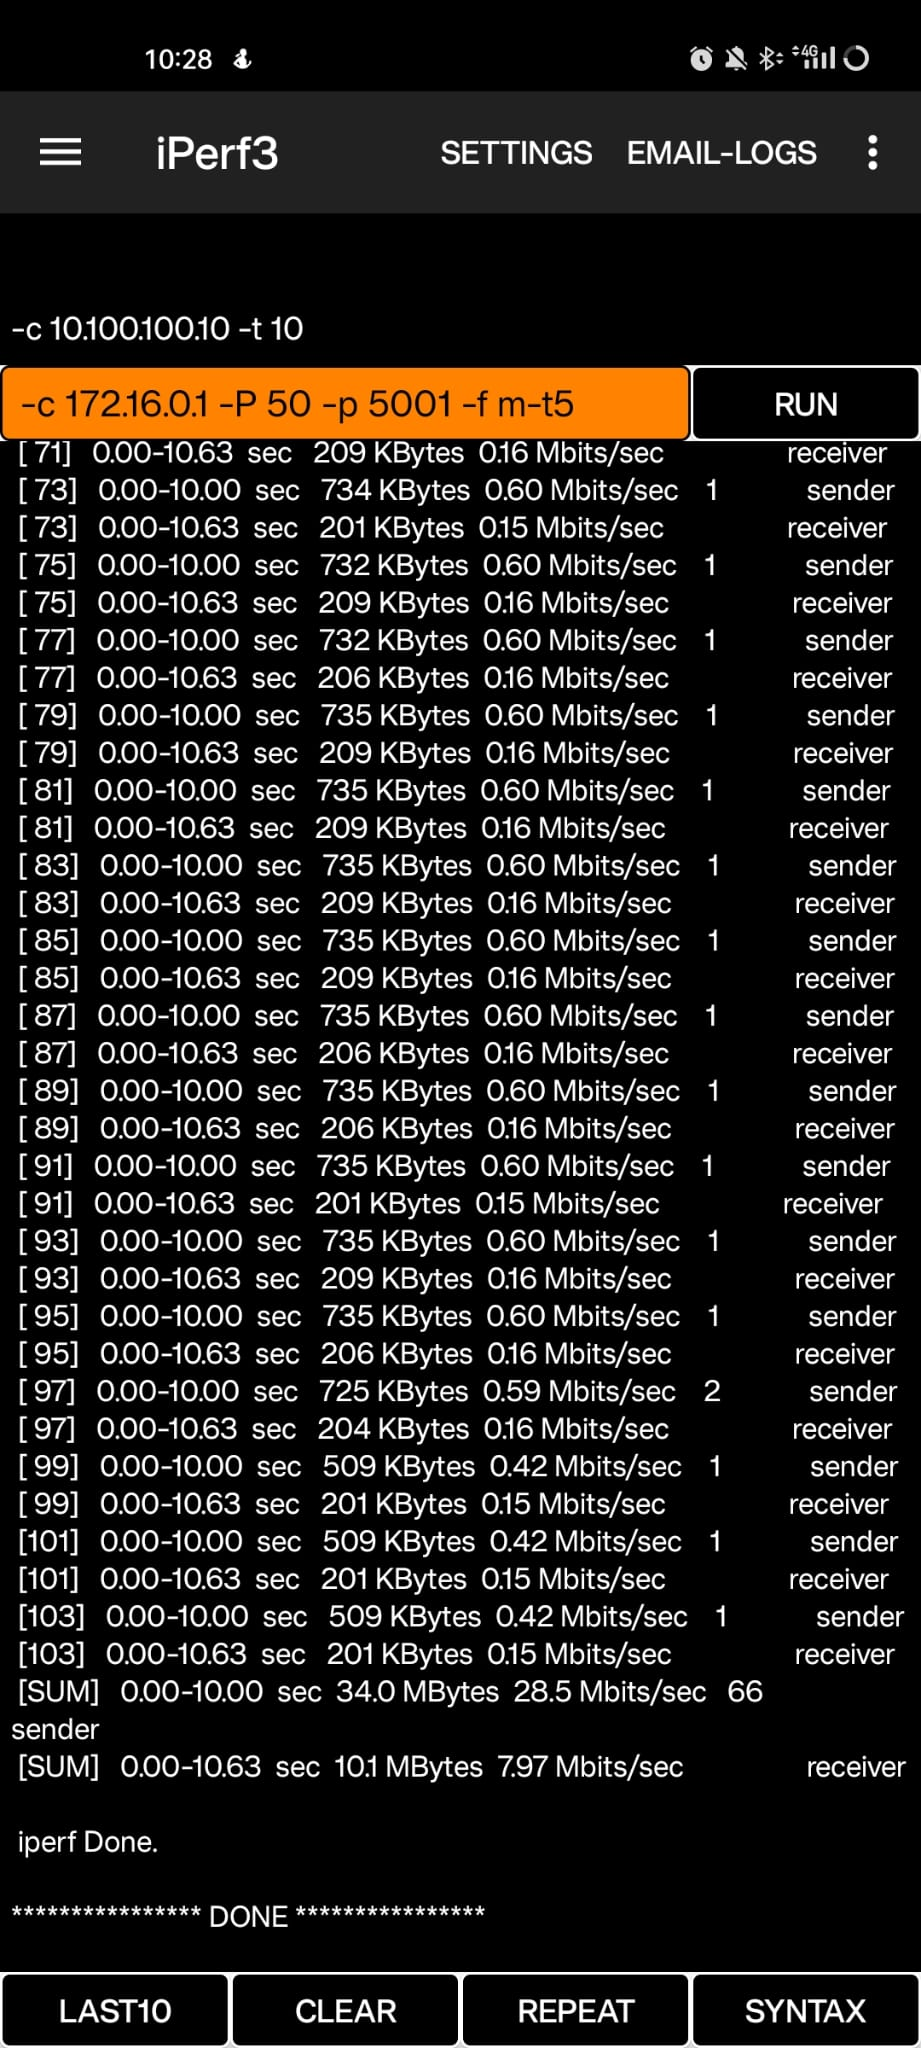
\includegraphics[width=0.35\linewidth]{Imagenes/Rendimiento/iperf3_2.jpeg}}
    \hspace{1.5cm}
    \subfloat{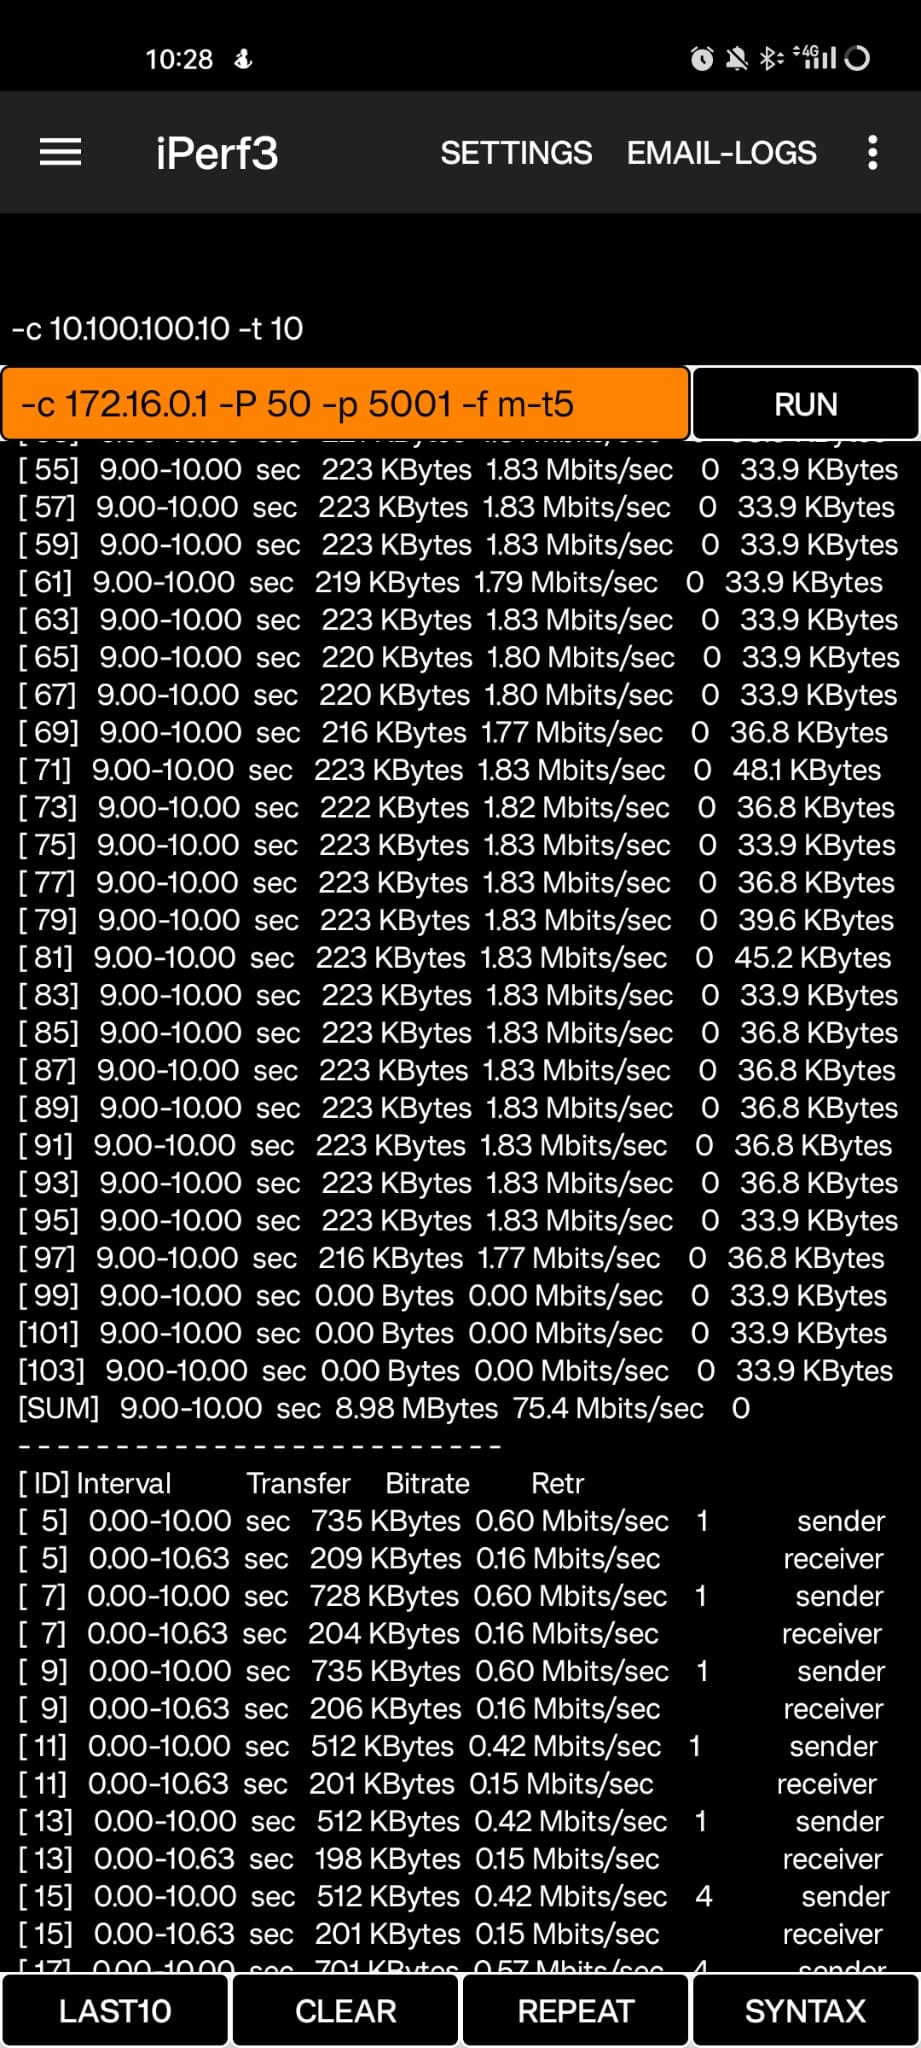
\includegraphics[width=0.35\linewidth]{Imagenes/Rendimiento/iperf3_1.jpeg}}
    \caption{Salida del comando ''iperf'' en el lado cliente.}
\end{figure}

\begin{lstlisting}[caption={Salida del comando ''iperf'' en el lado servidor.}]
[SUM]   0.00-1.00   sec   684 KBytes  5.61 Mbits/sec 
[SUM]   1.00-2.00   sec   766 KBytes  6.28 Mbits/sec 
[SUM]   2.00-3.00   sec  1.07 MBytes  9.01 Mbits/sec     
[SUM]   3.00-4.00   sec  1.07 MBytes  8.95 Mbits/sec 
[SUM]   4.00-5.00   sec  1018 KBytes  8.34 Mbits/sec 
[SUM]   5.00-6.00   sec   810 KBytes  6.64 Mbits/sec 
[SUM]   6.00-7.00   sec   806 KBytes  6.60 Mbits/sec
[SUM]   7.00-8.00   sec  1.06 MBytes  8.92 Mbits/sec 
[SUM]   8.00-9.00   sec  1.11 MBytes  9.29 Mbits/sec  
[SUM]   9.00-10.00  sec  1.10 MBytes  9.24 Mbits/sec 
[SUM]  10.00-10.63  sec   718 KBytes  9.28 Mbits/sec 
\end{lstlisting}

La salida de \textit{Iperf} depende de muchos factores, como la calidad de la señal, la carga de la red, la capacidad de los dispositivos involucrados, entre otros.
En una red 4G, una salida razonable dependería de la configuración y las características específicas de la red y de los dispositivos utilizados. Sin embargo, como referencia general, en una red 4G se pueden esperar tasas de transferencia de datos de al menos 10-20 Mbps, y en algunos casos incluso mayores, dependiendo de la calidad de la señal y la configuración de la red. Por lo que los resultados obtenidos son buenos. 

En cuanto al rendimiento de la red, según \cite{Rendimiento}, para un valor de 100 prb de download, obtenemos 7,5 bits/Hz. Extrapolando a nuestra situación donde prb tiene un valor de 25, obtenemos una tasa binaria de 18,75Mbits de forma teórica. Sin embargo, en las capturas, sólo obtenemos un valor máximo de 9,28, esto puede ser debido a varias causas, entre las que encontramos: 

Sobrecarga de red: la velocidad de la red 4G puede variar según la cantidad de usuarios conectados simultáneamente en una determinada celda. Si la celda está congestionada debido a un alto número de usuarios, la velocidad de transferencia puede disminuir. Esto afecta en gran medida a  nuestro caso, ya que en la misma sala están montadas 4 redes 4G a la vez. 

Interferencia electromagnética: La interferencia de otros dispositivos electrónicos o estructuras físicas puede afectar la calidad de la señal y, por lo tanto, disminuir la velocidad de transferencia. Al encontrarnos en un laboratorio de docencia entre los que encontramos elementos como routers, antenas, ordenadores, etc. eso afecta considerablemente.

Continuando con el análisis del rendimiento de la red punto a punto, creamos un programa en python que utiliza el protocolo NTP para calcular el delay, el jitter y la latencia, utlizando como servidor NTP la dirección 130.206.3.166, que corresponde al servidor hora.rediris.es. En el Anexo \ref{} se observa el código empleado.

El protocolo NTP calcula la latencia y los otros parámetros midiendo el tiempo que tarda una petición de tiempo en ser enviada desde un cliente a un servidor NTP y la respuesta del servidor en ser recibida por el cliente, siendo los clientes las diferentes interfaces de nuestra red.

Para la interfaz s1c (127.0.1.1) obtenemos una latencia media de 0.057ms y un jitter de 0.0077ms.
Para la interfaz MME (127.0.1.100) obtenemos una latencia media de 0.051ms y un jitter de 0.0078ms.
Para la interfaz PGW (172.16.0.1) obtenemos una latencia media de 0.036ms y un jitter de 0.008ms.
Para la interfaz de la sim asignada (172.16.0.6) obtenemos una latencia mediad e 41.3ms y un jitter de 0.033ms. Obviamente estos datos son peores que los anteriores ya que las interfaces anteriores se encontraban en el mismo ordenador, mientras que esta actual se encuentra en un dispositivo móvil alejado aproximadamente un metro de la SDR.

Podemos observar que se obtiene una latencia lógica para una red 4G.

\begin{lstlisting}[caption={Salida del fichero python que calcula retardos entre interfaces.}]

tp1@tp1-desktop:~/servicios_cloud_deep_racer$ /bin/python3 /home/tp1/Escritorio/ntpyptp.py
Interfaz 127.0.1.1 - Latencia: 0.051 ms, Jitter: 0.01369619369506836 s
Interfaz 127.0.1.100 - Latencia: 0.036 ms, Jitter: 0.013817548751831055 s
Interfaz 172.16.0.1 - Latencia: 0.037 ms, Jitter: 0.014568805694580078 s
Interfaz 172.16.0.3 - Latencia: 107.0 ms, Jitter: 0.09294772148132324 s
Interfaz 172.16.0.4 - Latencia: 26.9 ms, Jitter: 0.012932538986206055 s
tp1@tp1-desktop:~/servicios_cloud_deep_racer$ /bin/python3 /home/tp1/Escritorio/ntpyptp.py
Interfaz 127.0.1.1 - Latencia: 0.055 ms, Jitter: 0.013919591903686523 s
Interfaz 127.0.1.100 - Latencia: 0.036 ms, Jitter: 0.013829231262207031 s
Interfaz 172.16.0.1 - Latencia: 0.034 ms, Jitter: 0.013852596282958984 s
Interfaz 172.16.0.3 - Latencia: 60.1 ms, Jitter: 0.04521584510803223 s
Interfaz 172.16.0.4 - Latencia: 22.2 ms, Jitter: 0.008130550384521484 s
tp1@tp1-desktop:~/servicios_cloud_deep_racer$ /bin/python3 /home/tp1/Escritorio/ntpyptp.py
Interfaz 127.0.1.1 - Latencia: 0.041 ms, Jitter: 0.01411890983581543 s
Interfaz 127.0.1.100 - Latencia: 0.039 ms, Jitter: 0.014233112335205078 s
Interfaz 172.16.0.1 - Latencia: 0.045 ms, Jitter: 0.01401066780090332 s
Interfaz 172.16.0.3 - Latencia: 63.6 ms, Jitter: 0.04976511001586914 s
Interfaz 172.16.0.4 - Latencia: 23.4 ms, Jitter: 0.009380340576171875 s
tp1@tp1-desktop:~/servicios_cloud_deep_racer$ /bin/python3 /home/tp1/Escritorio/ntpyptp.py
Interfaz 127.0.1.1 - Latencia: 0.038 ms, Jitter: 0.014064311981201172 s
Interfaz 127.0.1.100 - Latencia: 0.049 ms, Jitter: 0.014048337936401367 s
Interfaz 172.16.0.1 - Latencia: 0.045 ms, Jitter: 0.013978242874145508 s
Interfaz 172.16.0.3 - Latencia: 62.4 ms, Jitter: 0.048295021057128906 s
Interfaz 172.16.0.4 - Latencia: 23.6 ms, Jitter: 0.009762048721313477 s
\end{lstlisting}

En general, se espera que la latencia entre interfaces internas de una red 4G sea bastante baja, ya que la comunicación entre los diferentes componentes de la red es esencial para proporcionar un servicio de alta calidad a los usuarios. En términos generales, se espera que la latencia entre interfaces internas en una red 4G sea inferior a 10 milisegundos (ms).

Latencia media extremo a extremo de una red 4G son 40ms


Como última de herramienta de análisis realizamos test de velocidad de internet mediante el test disponible en google.
Obtenemos una velocidad de descarga de 44.5 Mb/s y de subida de 21.1 Mb/s. Para un streaming de video en alta definición (HD) se esperan unas velocidades de bajada recomendadas de al menos 5 Mbps. y unas velocidades de subida recomendadas de al menos 5 Mbps.


\section{Kernel de Baja Latencia}

Para mejorar los resultados de rendimiento de la red instalamos el kernel de baja latencia de Linux y cambiamos las prioridades para que el núcleo tenga prioridad. Para ello utilizamos el comando:
\begin{verbatim}
sudo apt-get install -y linux-lowlatency.
\end{verbatim}
Por último, reiniciamos el ordenador y elegimos al arrancar el Linux de baja latencia.

En general los resultados obtenidos son bastante parecidos a los obtenidos con el kernel normal, con alguna excepción en el que mejora dicha latencia y ''Jitter''. 

\begin{lstlisting}[caption={Salida del fichero python que calcula retardos entre interfaces con kernel de baja latencia.}]
Interfaz 127.0.1.1 - Latencia: 0.041 ms, Jitter: 0.05975532531738281 s
Interfaz 127.0.1.100 - Latencia: 0.037 ms, Jitter: 0.05958867073059082 s
Interfaz 172.16.0.1 - Latencia: 0.036 ms, Jitter: 0.0597078800201416 s
Interfaz 172.16.0.2 - Latencia: 40.6 ms, Jitter: 0.019350528717041016 s
Interfaz 172.16.0.4 - Latencia: 45.8 ms, Jitter: 0.014258146286010742 s
\end{lstlisting}

Aún así se han realizado pruebas cuando la red no estaba muy congestionada, por lo que se espera que en una situación en en la que haya más usuarios usando la red, el rendimiento sea mejor usando un kernel de baja latencia que uno normal. 

